\documentclass[10pt,a4paper]{article}
\usepackage[utf8]{inputenc}
\usepackage[spanish]{babel}
\usepackage{amsmath}
\usepackage{amsfonts}
\usepackage{amssymb}
\usepackage{makeidx}
\usepackage{graphicx}
\usepackage{lmodern}
\usepackage{kpfonts}
\usepackage[left=2cm,right=2cm,top=2cm,bottom=2cm]{geometry}
\begin{document}
\begin{center}

\includegraphics[scale=0.2]{../Primer_Avance/Imagenes/upzmg.png} 
\end{center}
\paragraph{\Huge Primer Avance} \textbf{\Huge integrates:} \\ \\
	\begin{Large}
		Samuel Caleb Martinez Hernandez\\ \\
		Fabian Canales Ochoa\\ \\
		Amaury Efrain Gutierrez Chavez\\ \\
		Cesar Fabian Flores Macias\\ \\
		\end{Large}
		
	
\textbf{\Huge Materia:}\\ \\
		{\Large Cinemática de Robots}\\ \\
	
{\Huge \textbf{Nombre del Proyecto}:}\\ \\
		\textbf{\Large Brazo SCARA}
		
\section{Introduccion}
{\Large Esta tesis presenta una investigación en el 			diseño mecánico, modelado y control de un 				brazo robótico tipo SCARA de tres grados de 			libertad para ser empleado en algún proceso o 			actividad útil en la sociedad, ademas de tomar 			algunas consideraciones sobre su proceso de 			fabricación.} \\ \\

\section{{\Huge Objetivo}}
{\Large Construir y programar un brazo SCARA con una funcionalidad útil.}\\ \\

\section{{\Huge Materiales}}
{\Large Por ser primer avance, este apartado quedara vació.}\\ \\	

\section{{\Huge Procedimiento}}
{\Large Se inicio con la idea de un robot SCARA de cuatro piezas ensambladas piramidal mente, con un total de tres piezas con un total de grados de libertad del 180 por ciento aproximadamente Los diseños fueron en 2D fueron realizados en autocat la primera parte son las tres partes del robot los diseños se muestran en la siguiente imagen (1.001).}\\ \\
\begin{center}
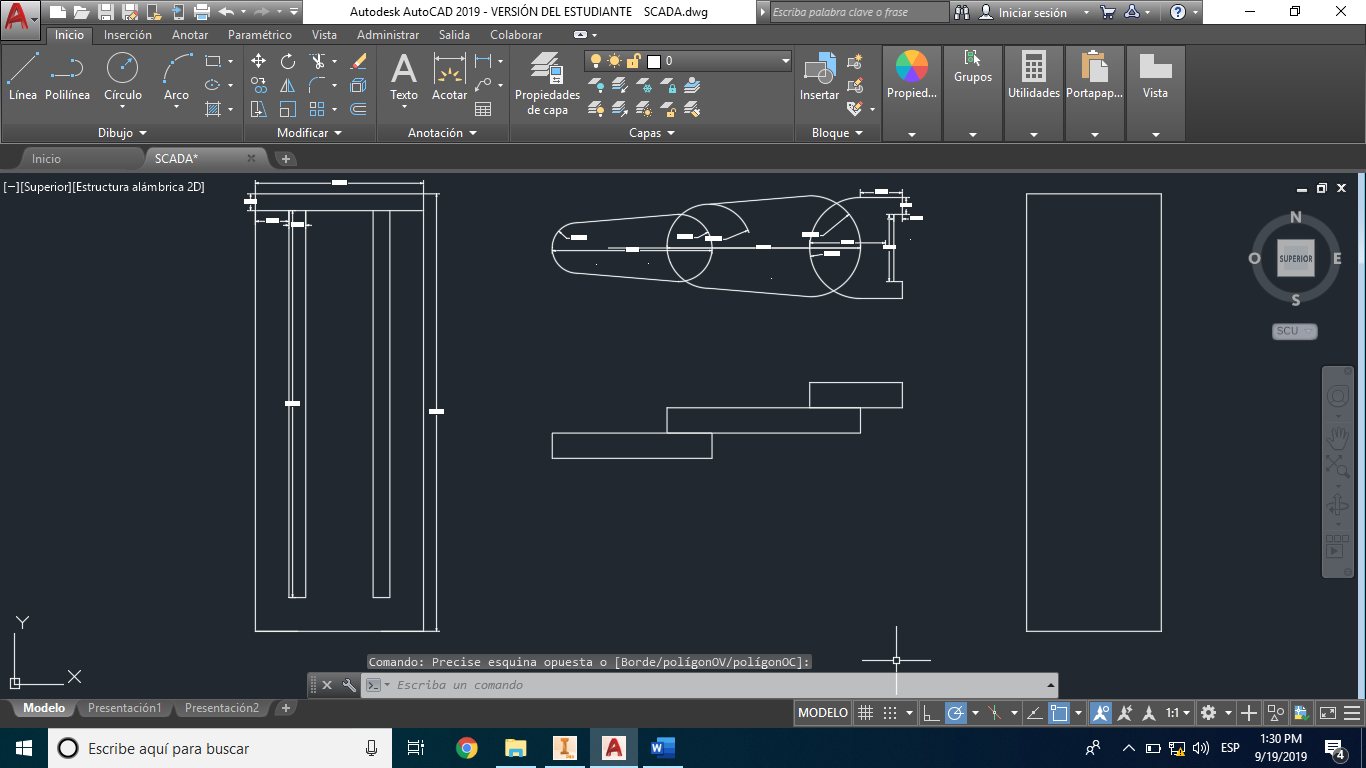
\includegraphics[scale=0.25]{Imagenes/2D.png} imagen 1.001  
\\{estos son los diseños en 2D se ve en dos ángulos las partes en una se ve la forma del robot ya que sera piramidal y en el otro angulo la forma de las partes.} \\ 
\end{center}

{\Large en la siguiente parte se realizaron los diseños en el programa inventor donde se muestran las partes principales del robot la siguiente imagen (1.002) sera la primera parte que salga de la base hay se nota el diseño que le dio:}\\ \\ \\
\begin{center}
 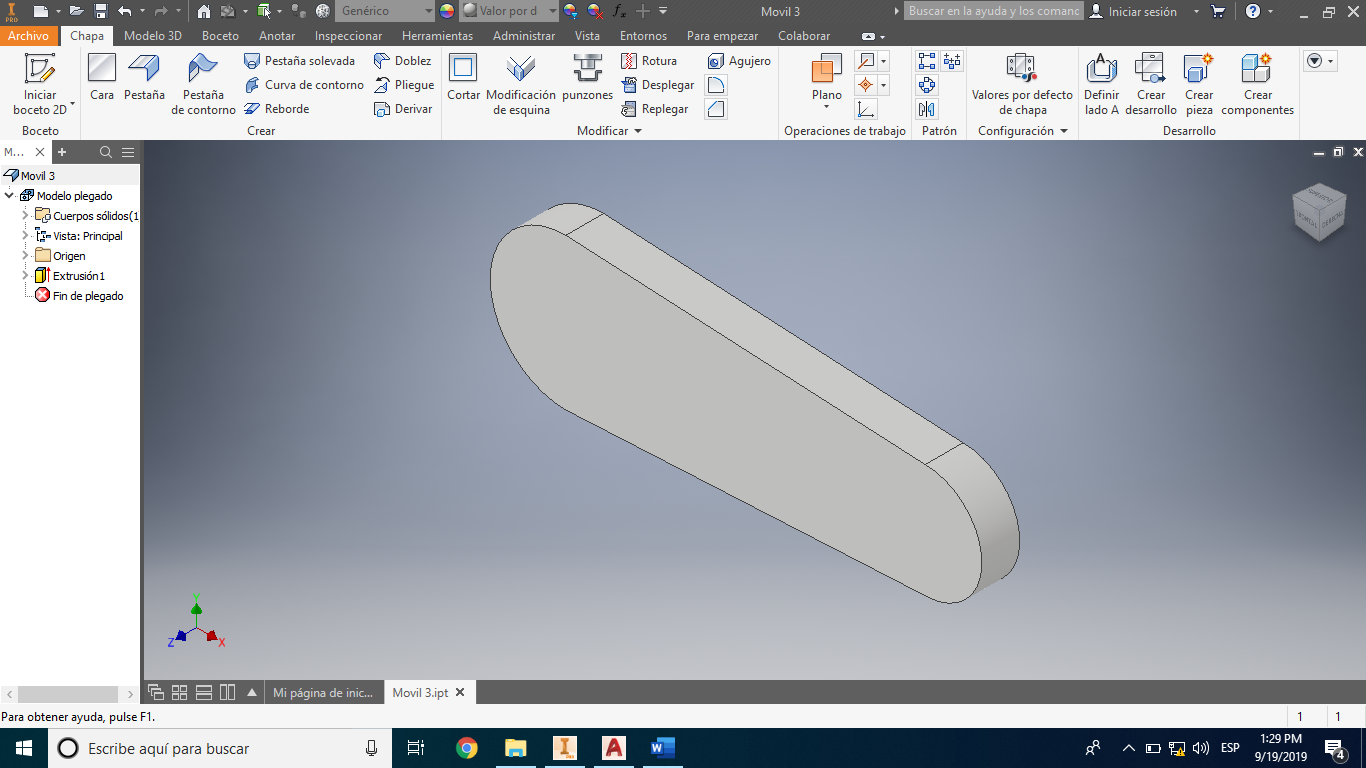
\includegraphics[scale=0.26]{../Primer_Avance/Imagenes/principal.png} {imagen 1.002  \\  se muestra el diseño curvo para facilitar en ensamble de las partes} \\

\end{center}
 {\large Como es de forma piramidal la forma siguiente la diseñmos mas pequeña para que no le gane el peso como se muestra en la imagen 1.003:
 \begin{center}
 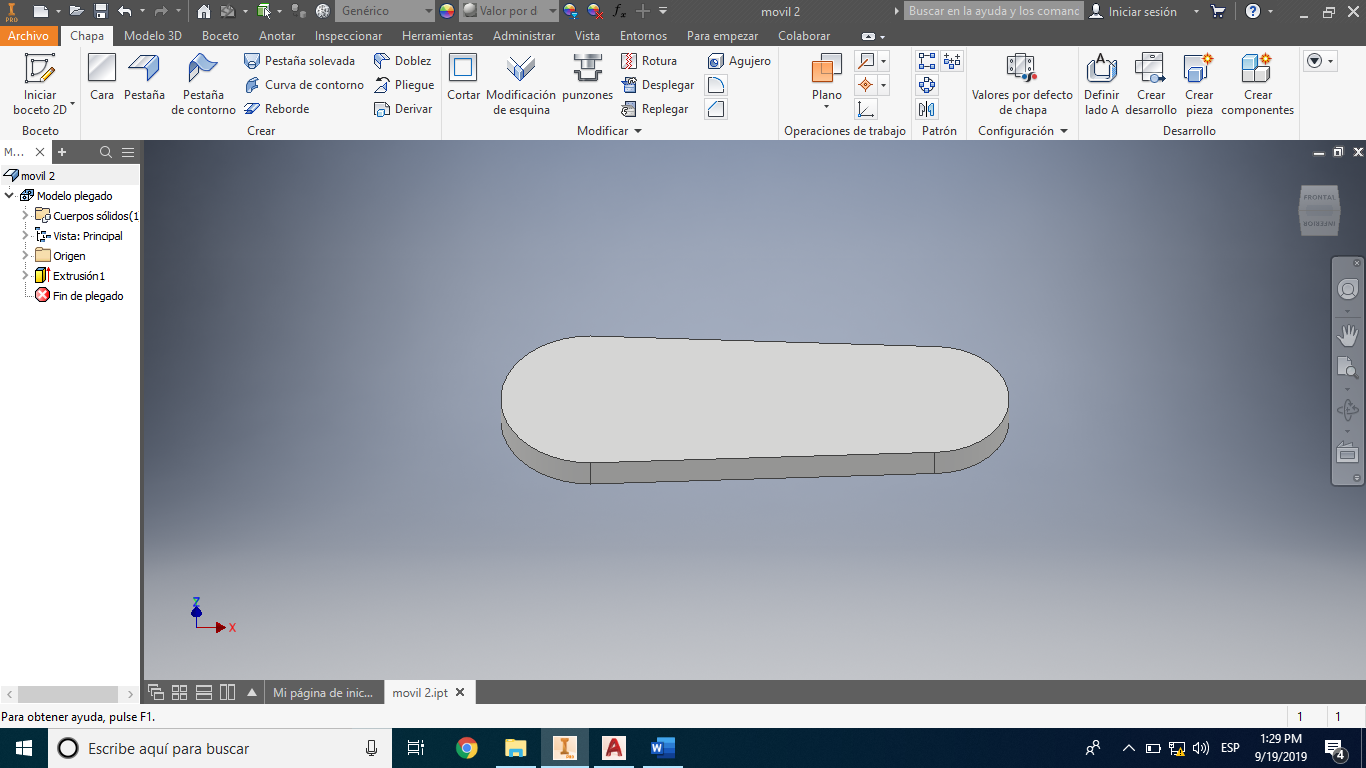
\includegraphics[scale=0.26]{../Primer_Avance/Imagenes/segunda.png} imagen 1.003 \\ 
 \end{center}
 \large Y ya por ultimo la tercera parte que planeamos que sea un diseño como pinza para que pueda sostener el peso requerido y sera la ultima parte como se muestra en la imagen 1.004;
 \begin{center}
 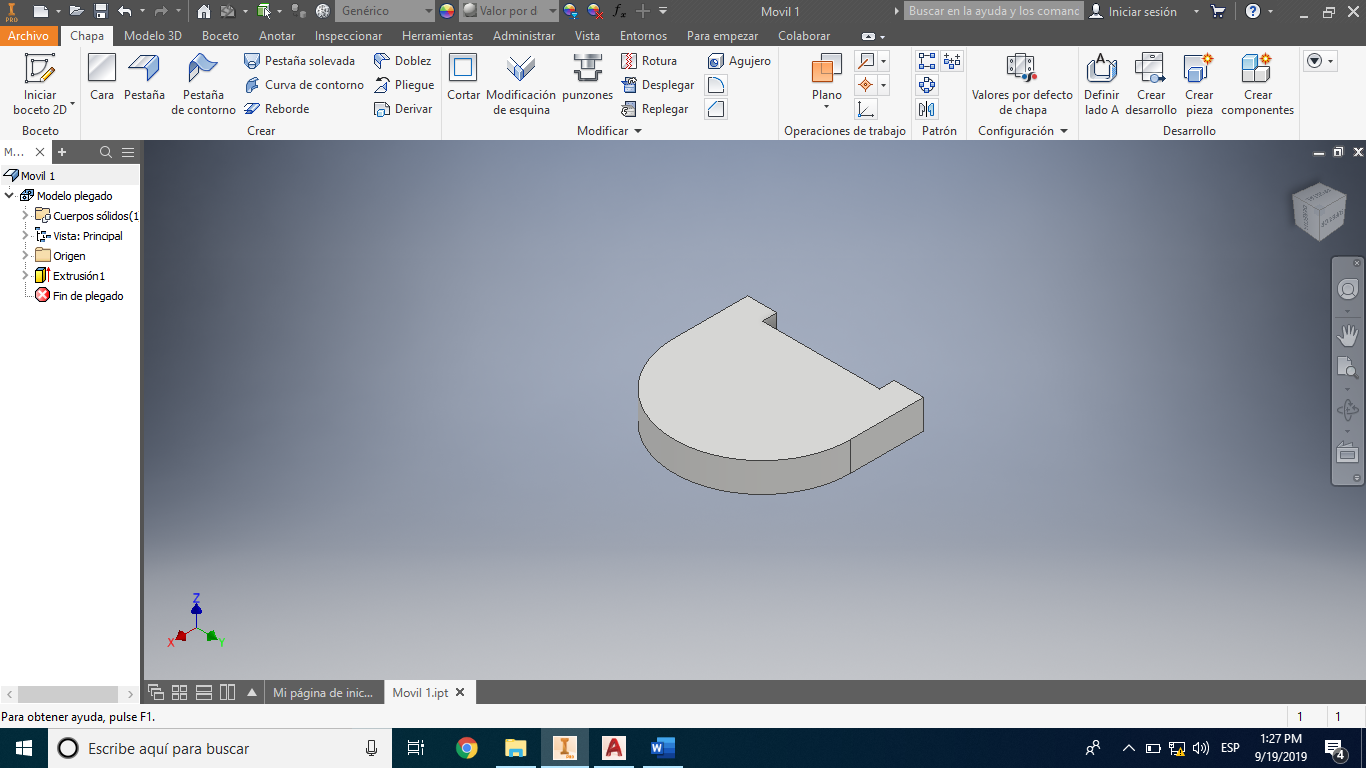
\includegraphics[scale=0.26]{../Primer_Avance/Imagenes/tercera.png}imagen 1.004
 \end{center}
 
\section{{\Huge Resultados }}

{\Large Eso esta por verse. }
\section{{\Huge Conclusiones }}
{\large Un robot SCADA siempre sera un reto para un estudiante sin importar que grado tenga, ya que  la mayoría de este tipo de robot esta con un 75 de matemáticas exactas para su buen funcionamiento, y tomando en cuenta los materiales a utilizar no solo sera un reto si no un aprendizaje del cual dejara muchos conocimientos que no pudiéramos haber imaginado.\\ \\ \\

En términos sencillos, cuando se trata de hacer que algo que puedes crear, tenga una utilidad, resulta bastante sencillo el poder crear una situación compleja donde la solución sea la creación en cuestión, en pocas palabras, el robot SCARA.\\ 
	
Los robots scara tienen una gran utilidad en la indurtria por su rapides y su precicion, ahora tenemos el reto de realizar un casi desde cero pero ahorita nomas hicimos el diseño en el que nos vamos a vasar, todavia nos falatan muchos pasos pero primero hay que comenzar por algo.\\ 

Para mi este es solo una pequeña parte solamente es el diseño del robot hay un largo camino   por recorrer lo bueno es que podemos mejorar cada diseño que realisamos para el robot aun nod faltan definir los materiales y hacer pruebas para ver la fuerza y si es que podra resistir los motores que sean mejores para que asi cumpla con los tres grados de libertad y que no se deforme el robot.
	
	
\end{document}